%\documentclass[conference]{IEEEtran}
\documentclass[11pt]{article}

\usepackage{fullpage}
\usepackage{graphicx}
\usepackage{wrapfig}
\usepackage{cite}

\begin{document}

\title{Qualifying Exam Research Proposal - Using Deep Learning Computer Vision Methods for Animal Re-identification from Camera Trap Data}

\author{Stefan Schneider}

\maketitle

\textbf{Abstract} - The ability of a researcher to re-identify (re-ID) an individual animal upon re-encounter is fundamental for addressing a broad range of questions in the study of ecosystem function, community and population dynamics, and behavioural ecology. Ecologists use a variety of methods for re-ID including tagging, scarring, DNA analyses, and camera traps. Tagging animals during mark and recapture studies is the most common method for reliable animal re-ID. However, this method can be laborious, intrusive, and expensive. Camera traps and video is a desirable alternative, requiring less labour, much less intrusion, and prolonged and continuous monitoring into an environment. Despite these advantages, the analyses of camera traps and video for re-ID by humans are criticized for their biases related to human judgment and inconsistencies between analyses. For decades ecologists with expertise in computer vision have successfully utilized feature engineering to extract meaningful features from camera trap images to improve the statistical rigor of individual comparisons and remove human bias from their camera trap analyses. Recent years have witnessed the emergence of deep learning systems which learn meaningful features from large data volumes. Current deep learning systems have demonstrated the accurate re-ID of humans based on image and video data with near perfect accuracy. Despite this success, few ecologists have utilized these approaches for animal re-ID. By utilizing novel deep learning methods for object detection and similarity comparisons, ecologists can extract animals from an image/video data and train deep learning classifiers to re-ID animal individuals beyond the capabilities of a human observer. This methodology will allow ecologists with camera/video trap data to re-identify individuals that exit and re-enter the camera frame. For this proposal, I will provide a brief history of camera traps for re-ID, present a collection of computer vision feature engineering methodologies previously used for animal re-ID, provide an introduction to the underlying mechanisms of deep learning relevant to animal re-ID, highlight the success of deep learning methods for human re-ID, describe the few ecological studies currently utilizing deep learning for camera trap analyses, describe the detailed methodology I propose for my research, my results thus far, and close with my predictions for near future methodologies based on the rapid development of deep learning methods.
\newline
\\
\textbf{Index Terms} - Animal Re-Identification, Camera Traps, Computer Vision, Convolutional Networks, Deep Learning, Density Estimation, Object Detection, Population Dynamics
\newline
\\
\noindent
%\begin{center}
%Key Words - Camera Traps, Computer Vision, Deep Learning, Machine Learning, Object Detection, Population %Monitoring,
%Word Count - 6,627
%\end{center}

\newpage

%\twocolumn
\section*{Introduction}

The ability to re-identify individual animals allows for population estimates to be used in a variety of ecological metrics including diversity, evenness, richness, relative abundance distribution, and carrying capacity, which contribute to larger, overarching ecological interpretations of trophic interactions and population dynamics \cite{whittaker1972evolution, hawley1982ecology, krebs1989ecological}. Ecologists have used a variety of techniques for re-ID including tagging, scarring, banding, and DNA analyses of hair follicles or feces \cite{krebs1989ecological, mowat2000estimating}. While accurate, these techniques are laborious for the field research team, intrusive to the animal, and often expensive for the researcher.
\newline
\\
Camera traps provide an alternative approach to animal re-ID by capturing photos in response to motion, or by continually recording video using weather-proof cameras in strategic locations \cite{o2010camera}. Compared to traditional methods of field observations, camera traps are desirable due to their lower cost and reduced workload for field researchers. Camera traps also provide a unique advantage by recording the undisturbed behaviours of animals within their environment. This has resulted in the discovery of surprising ecological interactions, habitat ranges, and social dynamics, among other insights \cite{stojanovic2014discovery, sangay2014wildife, scheel2017second, meek2013reliability}. 
\newline
\\
Despite these advantages, there are a number of practical and methodological challenges associated with the use of camera traps for animal re-ID. The discrimination of individual animals is often an expert skill requiring a considerable amount of training. Even among experienced researchers there remains the possibility for human error. Indeed, because of their lack of conspicuous features, some animals are difficult for experts to discriminate at the species level let alone among individuals of the same species \cite{meek2013reliability}. Historically, these limitations have restricted the use of camera traps for re-ID of animals that can either be easily and reliably tagged, or, that bear conspicuous individual markings. 
\newline
\\
One strategy for overcoming these limitations has involved the use of computer vision to standardize the statistical analysis of animal re-ID. The most widely used computational technique involves the use of `feature engineering' to design and implement algorithms that focus exclusively on pre-determined traits, such as patterns of spots or stripes, to discriminate among individuals. The main limitations of this approach surround its impracticality \cite{hiby2009tiger}. Feature engineering requires programming experience to design algorithms for feature extraction. It also requires sufficient familiarity with the organisms to identify relevant features. A further limitation of this approach is its lack of generality: once a feature detection algorithm has been designed for one species, it is unlikely to be useful for other taxa.  
\newline
\\ 
Recent decades have witnessed the emergence of deep learning systems that make use of large data volumes \cite{zheng2015scalable}. Modern deep learning systems no longer require `hard-coded' feature extraction methods. Instead, these algorithms can learn, through their exposure to large amounts of data, the particular features that allow for the discrimination of individuals. \cite{lecun2015deep}. These methods have been developed primarily outside the realm of ecology, first in the field of computer image recognition \cite{krizhevsky2012imagenet}, and more recently in the security and social media industries \cite{zheng2015scalable}. In this context, modern deep learning systems perform with higher accuracies than feature extraction and all other types of re-ID algorithms when trained on large amounts of data \cite{li2014deepreid, lisanti2015person, martinel2015re, zheng2016mars, xiaoend}. 
\newline
\\
In recent years, a handful of ecologists have begun utilizing deep learning systems for species and animal individual identification with great success \cite{norouzzadehautomatically, schneider2018deep, carter2014automated, freytag2016chimpanzee, brust2017towards, loos2013automated}. Our expectation is that this is just the beginning of a major trend that could revolutionize the analysis of camera trap data and, ultimately, our approach to animal ecology. In what follows, we first review the use of camera traps for animal re-ID, describing a collection of historic feature engineering approaches used for animal re-ID. Second, we provide a brief description of deep learning systems and the advances that have been made in the identification of human individuals. Our aim in this section is to introduce ecologists, who might be unfamiliar with these developments, to the basic strategies being employed by machine learning engineers to extract re-ID information from images and video. We then review the small number of examples in which deep learning has been used for species and animal identification. Finally, we conclude with some predictions and recommendations for near future implementations based on the rapid development of deep learning methods.

\section*{A Brief History of Camera Traps and Animal Re-Identification}

Animal photography was first introduced as a way of documenting the rare occurrence of seeing wildlife. While exploring South Africa in 1863, the German professor Gustav Fritsch is credited with the first successful attempt at photographing wild animals \cite{guggisberg1977early, kucera2011history}. In 1956, Gysel and Davis published the first work describing an automatic camera trap designed specifically for recording wildlife. It was a simple system where a camera was pointed at bait, which was wired to the camera, and when the animal ate the bait the camera would trigger \cite{gysel1956simple}. In 1959, Pearson developed a number of novel techniques for camera traps including camera triggers that were activated by foot plates and the interruption of a red laser, film documentation of animals utilizing a 16mm film movie reel, and animal re-ID in film by uniquely clipping the fur of captured animals \cite{pearson1959traffic}. Iterations of lighter and more portable cameras were developed over the years by Dodge and Snyder (1960) and Winkler and Adams (1968) for film recordings \cite{dodge1960automatic, winkler1968automatic}. In 1984, Seydack performed the first long term camera trap study leaving a camera in the South African rain forest for a month \cite{seydack1984application}. Seyback (1984) developed his own autonomous trip plate, winding wheel, and flash system for a 35mm camera and repeated the study six times over three years commenting on how the methodology will forever change ecological research \cite{seydack1984application}. In 1987, Hiby and Jeffrey demonstrated the unique advantage of the discrete nature of camera traps by documenting the Mediterranean monk seal (\textit{Monachus monachus}), a species highly sensitive to human disturbance \cite{hiby1987census}. In 1991, Carthew and Slater improved camera motion detection by introducing a pulse infrared beam as a trigger and, in 1994, Mace et al., combined microwave motion with passive infrared heat sensors to act as a trigger \cite{carthew1991monitoring, mace1994estimating}. In 1994, Mace et al.\ used their trigger system to provide one of the first population estimates based purely on camera trap data considering the abundance of grizzly bears (\textit{Ursus arctos}) \cite{mace1994estimating}. Due to the increased reliability of camera triggers and the decreased cost/size of cameras, camera traps became increasingly popular and more commonly used among ecological researchers. One such area was avian research, where numerous researchers took the opportunity to study nest predators \cite{laurance1994photographic, major1994inexpensive, leimgruber1994predation, danielson1996inexpensive} . For a more thorough and detailed synopsis of the history of camera traps see O'Connell et al. (2012) and/or Kucera and Barrett (2011) \cite{kucera2011history, o2010camera}. 
\newline
\\
Arguably the most influential researcher for camera trap re-ID methods is Karanth who used automated camera traps to photograph tigers (\textit{Panthera tigris}) in Nagarahole, India and estimate the tigers population density under a formal mark and recapture model \cite{karanth1995estimating, kucera2011history}. Since tigers are large, with obvious patterns/markings, humans can visually compare and identify individuals with reliable accuracy. The success of this study led to further experiments conducted in India by Karanth \cite{karanth1998estimation, karanth2004estimation} and influenced other researchers to follow Karanth's methodology of examining creatures with obvious markings, such as tigers \cite{o2003crouching, kawanishi2004conservation}, jaguars (\textit{Panthera onca}) \cite{silver2004assessing, silver2004use}, leopards (\textit{Panthera pardus}) \cite{henschel2003leopards}, and ocelots (\textit{Leopardus pardalis}) \cite{maffei2005ocelot, trolle2005camera}. Karanth et al. (2006) has since continued his study of Nagarahole tiger populations, and in 2006 released a 9-year study documented the estimated survival, recruitment, temporary emigration, transience, and rates of population change \cite{karanth2006assessing}. In 2008, Rowcliffe and Carbone documented a 50\% annual growth in publications using camera trap methods to assess population sizes between 1998 and 2008 and the trend has persisted until 2015 \cite{rowcliffe2008estimating, burton2015wildlife}. 
\newline
\\
Camera traps are desirable as they have reduced manual labour dependencies, cheaper cost, and provide additional insight into environmental interactions compared to traditional field observations \cite{henschel2003leopards, silveira2003camera, wegge2004effects}. Population estimates using camera traps are often performed calculating the Lincoln-Peterson index which assumes that individuals are accurately re-identified \cite{southwood2009ecological}. As a result, despite the advantages of camera traps, re-ID is currently restricted to animals where each individual reliably has a distinct pattern/feature that a human observer can distinguish \cite{trolle2005camera}. Relatively few species have natural markings sufficiently variable to be individually recognizable. As a result most camera trap studies focus on spotted and striped felids, both of which can be discriminated at the individual level \cite{karanth1998estimation, henschel2003leopards, maffei2005ocelot}. This places a limitation on the range of viable species capable of being analyzed with this method and creates a bias where species without individual markings have been under-represented in recent camera trapping research \cite{trolle2003mammal, srbek2005camera}. Foster and Harmsen (2011) identify these limitations and others while reviewing and criticizing 47 camera trap population studies. They further note a potential source of bias stems from reserachers’ individual judgments about animal identity based on markings which are often subtle or difficult to perceive in the available images \cite{foster2012critique}.
\newline
\\
In order to standardize the analyses of individuals, ecologists with computer vision expertise developed a number of unique and creative feature engineering approaches to extract meaningful information from images of animals for the purpose of re-ID. We present a collection of these works here. 

\section*{Feature Extraction Methods for Animal Re-Identification}

Computer vision has been used as a tool for animal re-ID for decades. Here we outline the history of computer vision specific to animal re-ID, beginning with the earliest computer aided approaches, followed by manual feature extraction methods and the transition to more advanced models involving algorithmic feature engineering.  
\newline
\\
The first use of computer vision for animal re-ID was introduced in 1990 by Whitehead, Mizroch et al., and Hiby and Lovell who published collectively in the same journal \cite{whitehead1990computer, mizroch1990computer, hiby1990computer}. Whitehead (1990) considered sperm whales (\textit{Physeter macrocephalus}) using custom software to scan projector slides of a sperm whales fluke onto a digitizer tablet \cite{whitehead1990computer}. The user would manually tap the location of a unique characteristic (such as a nick or a scratch), provide a descriptive characteristic, and save the information to a database (Figure 1). When a unseen image is scanned, the user inputs the descriptive characteristics and the software considers the maximum sum of similarities to return the most similar individual. With a database of 1,015 individuals, 56 were tested returning a 32\% top-1 and 59\% top-10 accuracy \cite{whitehead1990computer}. Top-1 and top-10 accuracy are commonly reported metrics which describe the percent of accurate predictions in the first and top ten most confident outputs of a model respectively. Mizroch et al.\ (1990) considered humpback whales (\textit{Megaptera novaeangliae}) using customized software where the fluke was uploaded and the user labeled the image considering a 14-sector fluke map selecting from a list of possible markings (Spots, circles, missing, pigment, etc.). Results were compared using a similarity matrix and with a test set of 30 images the system returned a top-1 accuracy of 43\% \cite{mizroch1990computer}. Re-ID from images of the fluke of a whale remains a research interest today \cite{kagglehumpbackreid}. Lastly, Hiby and Lovell (1990) developed a system considering the grey seal (\textit{Halichoerus grypus}) where the user inputs numerous head captures of an animal from the same pose and the system renders a 3-D model of the animal \cite{hiby1990computer} (Figure 2). An individual's representation is captured in the summation of the grey scale pixel values of each `pattern cell' and considering a test set of 56 images, Hiby and Lovell report a 98\% top-1 accuracy using this model \cite{hiby1990computer}. In 1995, Dufault and Whitehead revisit the pigment and marking changes over time of sperm whales stating their databases must be updated otherwise individuals will be unrecognizable \cite{dufault1995assessment}. In 1998, O'Corry-Crowe compared the wavelet transformation of the fluke of sperm whales receiving a 92.0\% accuracy considering 56 images \cite{o1998identification}. 
\newline
\\

\begin{wrapfigure}{r}{0.5\textwidth}
  \begin{flushright}
    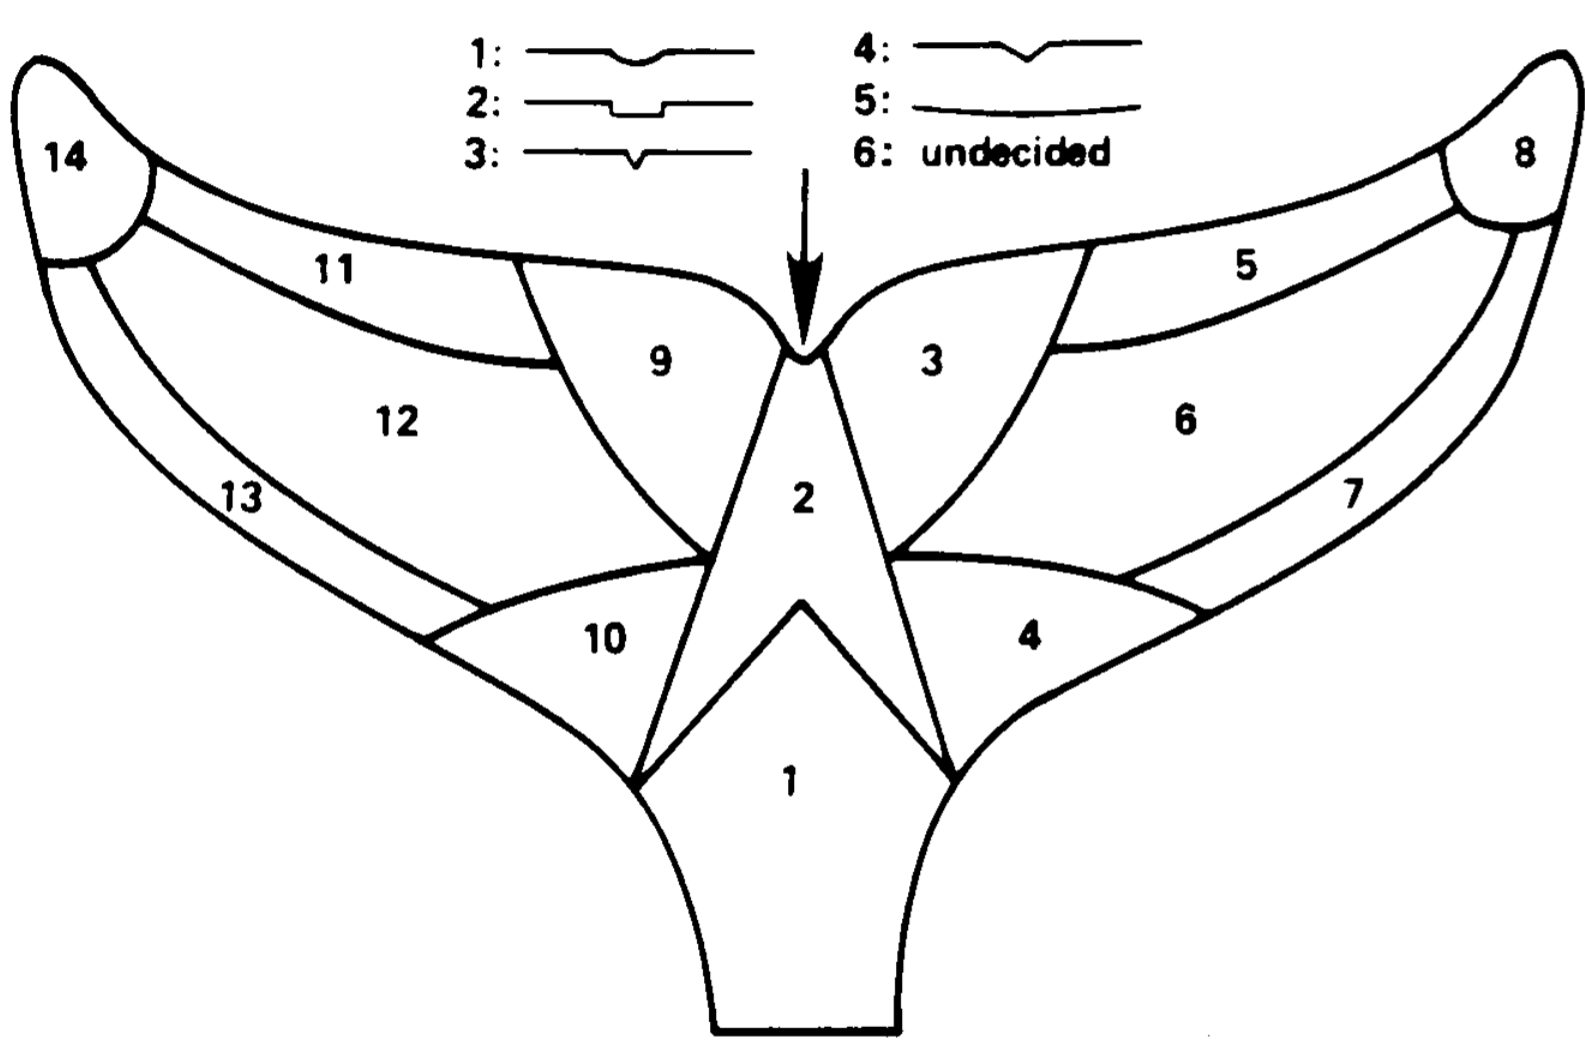
\includegraphics[width=3in]{FlukeMap.png}
  \end{flushright}
  \caption{Example of the fluke mark mappings used by Mizroch et al. (1990).}
\end{wrapfigure}

\noindent
Using computer vision for re-ID increased in popularity in the 2000s when Kelly (2001) used the same 3-D model approach as Hiby and Lovell (1990), comparing the collective similarity of pattern cells of cheetahs (\textit{Acinonyx jubatus}) \cite{kelly2001computer, hiby1990computer}. Kelly (2001) achieved a 97.5\% top-1 accuracy considering 10,000 images without describing a train/test distribution, commenting that this technique could potentially work for many ungulate and cat species, provided that it has access to high quality images \cite{kelly2001computer}. In 2003, Hillman et al., developed an autonomous feature extraction method to capture unique nicks, scratches, and markings from the dorsal fin of six whale and dolphin species \cite{hillman2003computer}. Named \textit{Finscan}, the system localized 300 xy pairs from each fin and determined individual similarity by calculating the Euclidean distance of these pairs and returning the minimum distance to represent similarity \cite{hillman2003computer}. Hillman et al. (2003) report accurate classification results of 50\% top-1 and 75\% top-4 accuracy \cite{hillman2003computer}. 
\newline
\\
The complexity of feature extraction increased in 2004 as Ravela and Gamble used a Taylor approximation of local colour intensities, multi-scale brightness histograms, and curvature/orientation to re-ID marbled salamander (\textit{Ambystoma opacum}) individuals using a normalized cross-covariance \cite{ravela2004recognizing}. Ravela and Gamble (2004) constructed a custom housing for their camera trap with four walls, single coloured floor, and a motion camera to capture top down images of salamanders as they entered. A database of 370 individuals was gathered and considering a test set of 69 queries the method returned a top-1 accuracy of 72\% \cite{ravela2004recognizing}. In 2005, Arzoumanian et al.\ explored whale shark (\textit{Rhincodon typus}) re-ID by analyzing the characteristic flank (front dorsal region) spot patterns using an astronomy algorithm for recognizing star patterns \cite{groth1986pattern, arzoumanian2005astronomical}. The algorithm creates a list of possible triangles from white dots within an image using xy pairs and compares their orientation between images. Arzoumanian et al.\ (2005) tested 236 images of individuals and report a top-1 accuracy of 90\%. They claim their incorrect results are mainly a result of poor image quality \cite{arzoumanian2005astronomical}. In 2007, Ardovini et al.\ attempted to re-identify elephants  \textit{Loxodonta spp.} without specifying species based on images using a multi-curve matching technique where a spline curve is fit to the mantle of an individual elephant \cite{ardovini2008identifying}. To re-ID an elephant, the known spline curves were overlaid atop the image of the elephant and the most similar was considered the same individual \cite{ardovini2008identifying}. The researchers report a 75\% top-1 accuracy utilizing this technique considering 200 test images and the methodology has been used by the Centre for African Conservation \cite{ardovini2008identifying}.
\newline

\begin{wrapfigure}{r}{0.5\textwidth}
  \begin{flushright}
    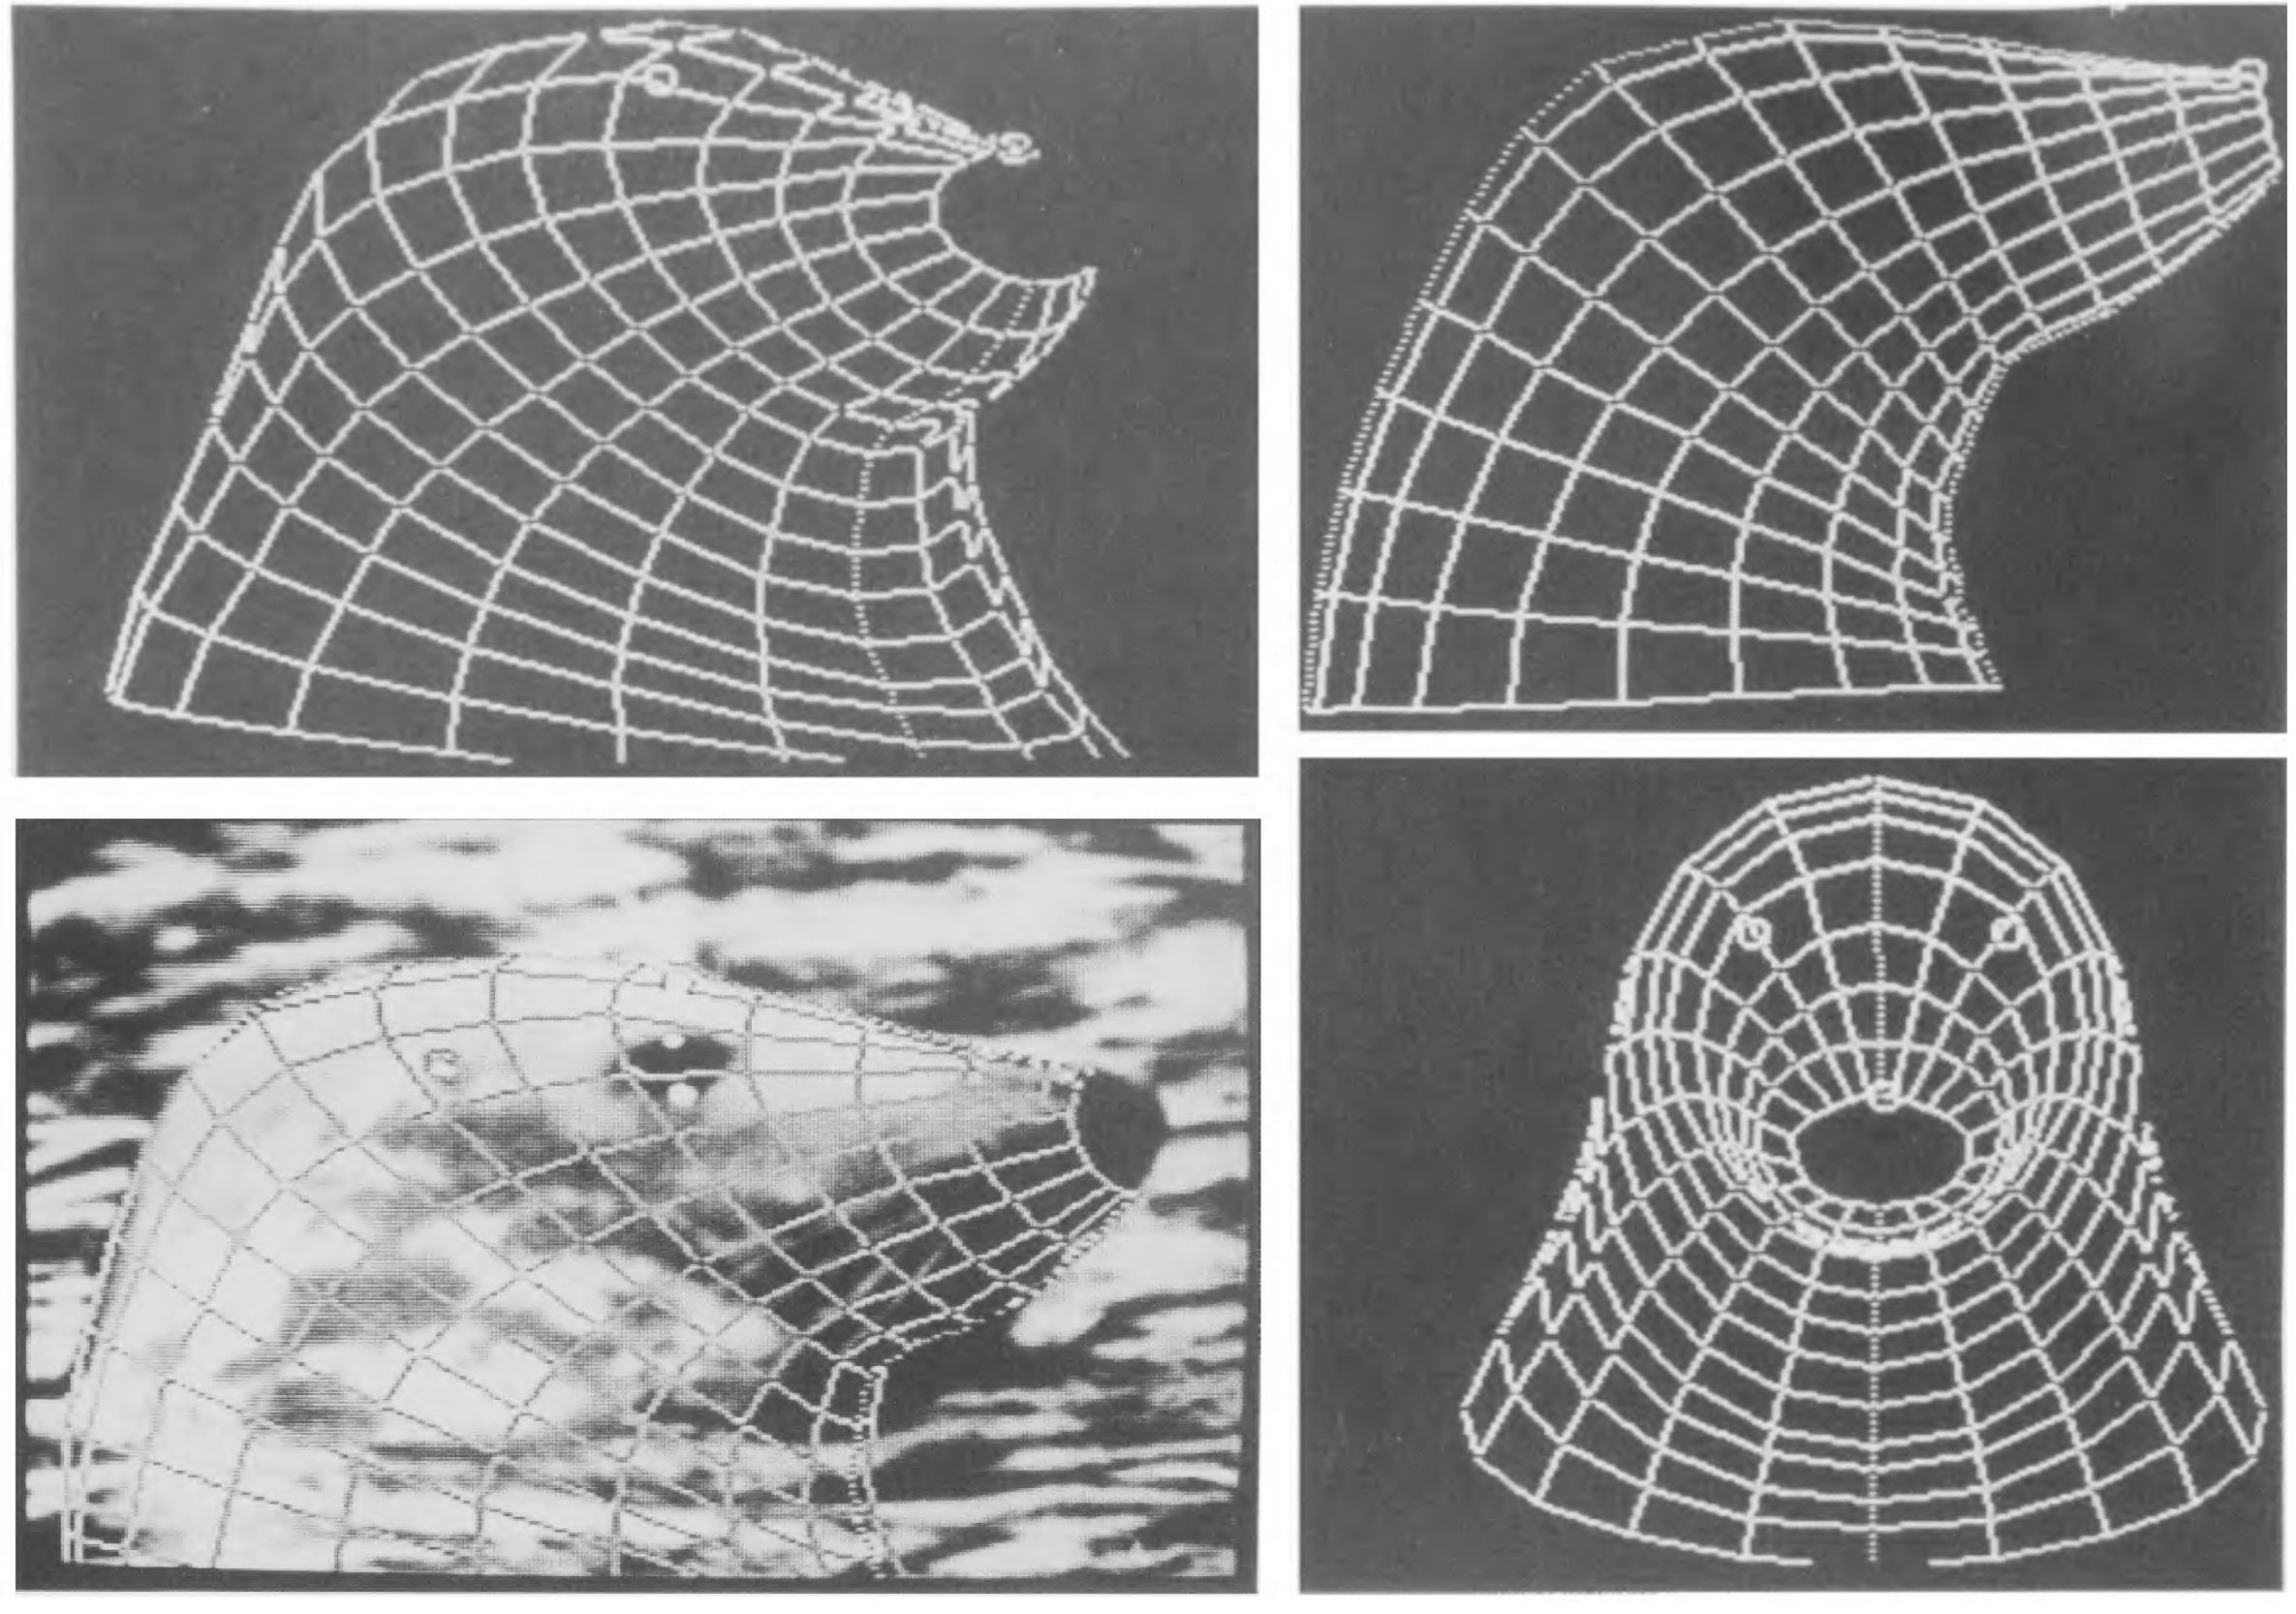
\includegraphics[width=3in]{SealWireFrame.png}
  \end{flushright}
  \caption{Example of the 3-D models generated by Hiby and Lovell (1990).}
\end{wrapfigure}

\noindent
The first computer vision model for animal re-ID capable of generalizing across species was developed in 2007 by Burghardt and Campbell which extracted inherent singularities (spots, lines, etc.) of animal individuals \cite{burghardt2007fully}. The technique involves three cameras pointed at a central location to capture a 3-D representation of the animal and extracts features using Haar-like (pixel difference) descriptors. For each feature, an AdaBoost classifier was trained to determine if the single feature was present or not and individual re-ID governed by an ensemble of these features \cite{burghardt2007fully}. In 2010, Sherley et al. used this approach on Robben Island, Africa in one of the first works to perform fully autonomous population estimates solely from camera traps considering the African penguin (\textit{Spheniscus demersus}) \cite{sherley2010spotting}. Considering numerous trials, the system returned an accuracy between 92-97\% in comparison to records from humans on site \cite{sherley2010spotting}. 
\newline
\\
In 2009, Hiby et al. collaborated with Karanath to explore their 3-D model representation technique considering his long term tiger population studies \cite{hiby2009tiger}. By again dividing individuals into pattern cells, re-ID was considered by the summation of the similarity of the cells were considered using a Bayesian posterior probability estimate and tested considering live tigers and poached tiger rugs (Figure 3). Hiby et al.\ (2009) report a 95\% and 100\% top-1 and top-5 accuracy considering 298 individuals \cite{hiby2009tiger}. In 2011, Lahiri et al.\ attempted to differentiate between zebra (\textit{Equus zebra}) individuals by dividing the image into rows and comparing a histogram representation of pixel values for different individuals \cite{lahiri2011biometric}. Lahiri et al.\ (2011) report a top-1 accuracy of 50\% when considering 85 individuals \cite{lahiri2011biometric}. The popularized Scale-Invariant Feature Transformation (SIFT) algorithm was used by Bolgar et al.\ (2012) to extract distinctive features, such as colour distribution, from a population of Masai giraffe (\textit{Giraffa camelopardalis tippelskirchi}) \cite{bolger2012computer}. Bolgar et al.\ (2012) compare estimated population size of the giraffe population with manual mark and recapture methodology and claim their model returns a similar population estimate without providing a numeric value \cite{bolger2012computer}. 
\newline

\begin{wrapfigure}{r}{0.5\textwidth}
  \begin{flushright}
    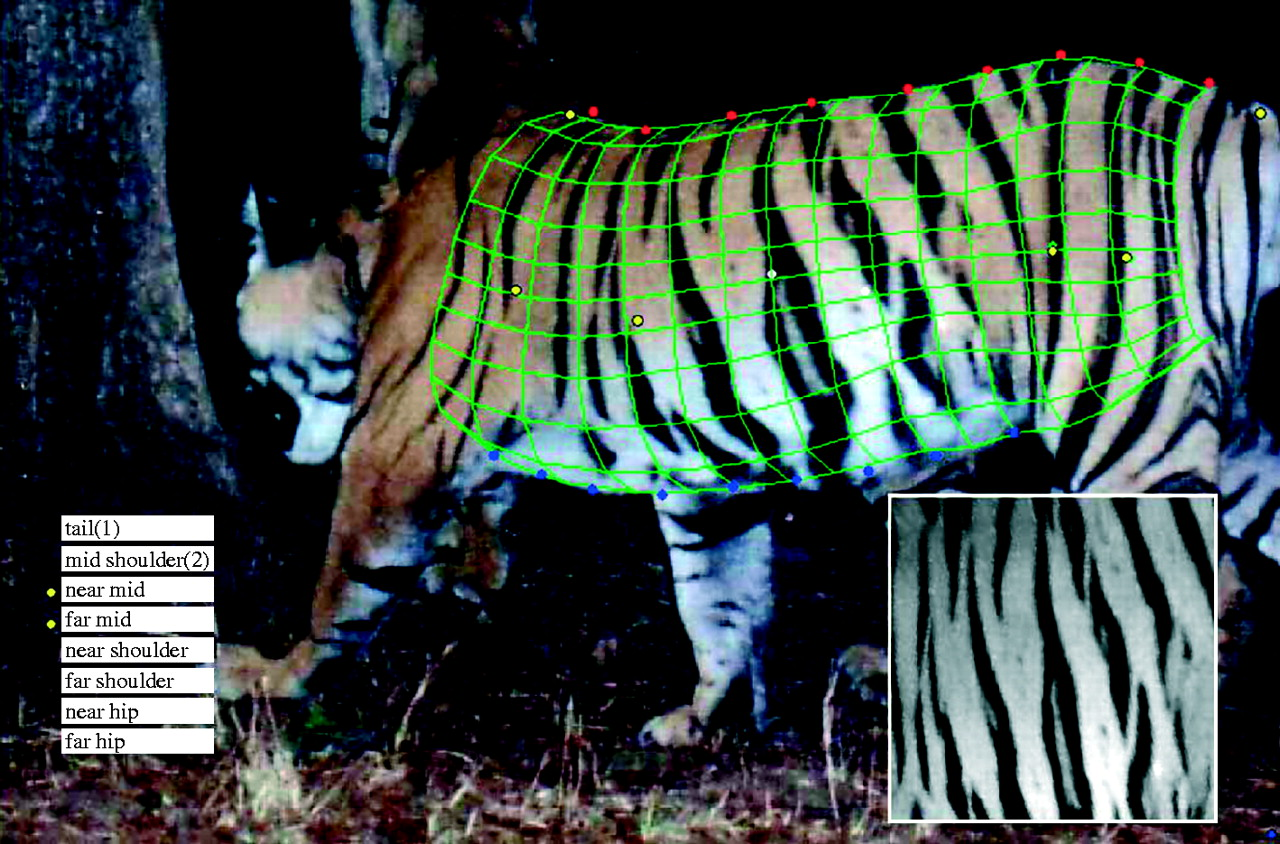
\includegraphics[width=3in]{3DTiger.jpg}
  \end{flushright}
  \caption{Example of 3-D models generated by Hiby et al. using Karanth's tigers (Hiby et al., 2009)}
\end{wrapfigure}

\noindent
In 2013, Town et al.\ compared individual similarity of manta ray species (\textit{Manta alfredi} and \textit{Manta birostris}) based on images of their ventral side using the contrast-limited adaptive histogram equalization algorithm to enhance local contrasts and then compare colour histograms using a Gaussian filter \cite{town2013manta}. Considering 720 images, Town et al. report a 51\% and 68\% top-1 and top-10 accuracies, closing by describing the difficulties of blurriness, lighting difficulties, and colour disparities when working with underwater imagery \cite{town2013manta}. Also in 2013, Loos and Ernst attempt to re-ID the faces of chimpanzee \textit{Pan spp.} considering features composed of pixel value gradient changes and pixel groupings of similar intensity and then training a Support Vector Machine classifier. Loos and Ernst (2013) report an accuracy of 84.0\% and 68.8\% on their two labeled data sets, C-Zoo and C-Tai, which they have since made publicly available \cite{loos2013automated}. In 2017, Hughes and Burghardt developed a fully automated contour-based visual shark fin ID system and show that selective feature extraction from shark fins can successfully represent individuality \cite{hughes2017automated}. Using a fin contour feature extraction method creating representations of `fin space', Hughes and Burghardt (2017) propose a local naive Bayes nearest neighbour non-linear model for individual animal recognition \cite{hughes2017automated}. Their approach returns a top-1 accuracy of 82\% for correctly classified shark individuals, and a 91\% top-10 accuracy considering 2,371 images.
\newline
\\
While these techniques have shown success, there remain areas of improvement for the performance, design, implementation and accessibility when using computer vision for animal re-ID (Table 1). 

\section*{Deep Learning and Its Success for Human Re-Identification}

Modern deep learning systems have shown great success learning the necessary features for re-ID from data and removes the need for feature engineering. Deep learning as concept originated in the 1940-1960s as cybernetics, was rebranded as connectionism between 1980 and 1995, and starting in 2006 rebranded again as deep learning \cite{mcculloch1943logical, hebb2005organization, minsky2017perceptrons, rumelhart1986learning, hinton2006fast}. Despite its long history, there has been a rapid growth of interest in deep learning due to improved computational power and the availability of large data sets, both requirements for the model. In recent years, deep learning methods have dramatically improved performance levels in the fields of speech recognition, object recognition/detection, drug discovery, genomics, and other areas. It has become the standard computational approach for problems with large amounts of data \cite{lecun2015deep}. Here, we provide a brief description of the underlying mechanism of deep learning as it relates to computer vision and animal re-ID. The process that will be outlined in this section is an approach known as supervised learning and is the most common form of deep learning \cite{lecun2015deep}. Other forms include unsupervised problems (eg. clustering, generative adversarial networks), reinforcement learning (eg. deep Q-networks), compression (autoencoders), among others \cite{goodfellow2016deep}. For additional details on deep learning we refer the reader to `Deep Learning', `Deep Learning in Neural Networks: An Overview', and/or the text `Deep Learning' \cite{lecun2015deep, schmidhuber2015deep, goodfellow2016deep}(Goodfellow et al., 2016).
\newline

\begin{wrapfigure}{r}{0.5\textwidth}
  \begin{flushright}
    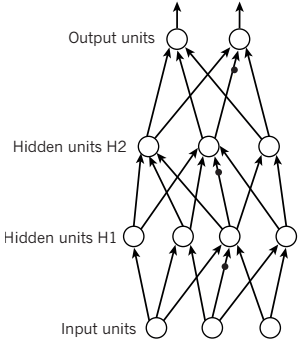
\includegraphics[width=3in]{BasicNeuralNet.png}
  \end{flushright}
  \caption{Condensed example of a neural network. Deep neural networks can have millions of weights per layer and dozens of layers (LeCun et al., 2015)}
\end{wrapfigure}

\noindent
Deep learning is a computational framework where a system's parameters are not designed by human engineers but trained from large amounts of data using a general-purpose learning algorithm \cite{lecun2015deep}. Intuitively, deep learning systems are organized as a layered web/graph structure where labeled data are submitted as input, and many modifiable scalar variables (known as weights) are summed and multiplied by a non-linear transformations to output a predicted label from a predefined number of possible choices \cite{goodfellow2016deep}. Each training example is fed through the network providing an answer, and based on the results from an `objective function', (ie. the average answer accuracy across the data set) the weight values are modified by an optimizer (e.g. gradient descent with backpropagation) in an attempt to improve accuracy \cite{goodfellow2016deep}. Deep learning systems will often have millions of modifiable weight values and with enough data and computation, the underlying relationship between the data and output can be mapped to return accurate results \cite{krizhevsky2012imagenet, simonyan2014very, szegedy2015going, he2016deep}. The general term for this framework is a neural network of which there are many architectures (Figure 4). The architecture described here is known as a feedfoward network \cite{lecun2015deep}. In 1991, Hornik proved feedforward neural networks are a universal approximator, capable of mapping any input to output if a relationship exists \cite{hornik1991approximation}.
\newline
\\
Neural networks are best described as multiple processing layers where each layer learns a representation of the data with different levels of abstraction \cite{lecun2015deep}. As the data representation passes through each transformation it allows for complex representations to be learned \cite{lecun2015deep}. Consider an example data set of many black and white images of animal individuals. The images are initially unravelled into a single vector of pixel values between 0 and 255 and fed into a deep learning system. Using this raw input the first layer is able to learn simple representations of patterns within the data, such as the presence or absence of edges at particular orientations and locations in the image. The second layer will typically represent particular arrangements of edges and open space. The third layer may assemble these edges into larger combinations that correspond to parts of familiar objects, such as the basics of a nose, or eyes, and subsequent layers would detect objects as combinations of these parts, such as a face \cite{lecun2015deep}. Based on the combination of larger parts, such as the ears, face, or nose, a learning system is able to correctly classify different individuals with near perfect accuracy when given enough input data \cite{swanson2015snapshot}. A deep learning system can learn the subtle details distinguishing a unique classification, such as a differing antler structure, and ignore large irrelevant variations such as the background, pose, lightning, and surrounding objects \cite{krizhevsky2012imagenet}.
\newline
\\
Due to the massive number of possible weight parameters deep learning models sometimes overfit, learning specific nuances relevant to its training data that are not generally transferable. To detect overfitting and measure a model's performance, before training a model, the data are randomly segregated into a training and test set where the test set is never shown to the model during training. The results of the model, and its ability to generalize to examples it has never seen, is based on its performance on the test set. Accuracy on the test set is a commonly used metric for performance, however this metric can provide a poor representation of a models capabilities when considering data with an unequal distribution of classifications. The F1 Score, introduced by Yang and Liu (1999), is also often included and considers the distribution of correct classifications by quantifying the precision (ratio of a correct classification prediction to the total predicted for that classification) and recall (ratio of correct classification predictions to the total number of the classification in the data) into a single representation using the formulation: \cite{yang1999re} $$F1=2*\frac{precision*recall}{precision+recall}$$
\newline
\\
Many recent advances in machine learning have come from improving the architectures of a neural network. One such architecture is the Convolutional Neural Network (CNN), first introduced as the `Neocognitron' in 1979 by Fukushima, which is now the most commonly used architecture for computer vision tasks today \cite{fukushima1979neural, krizhevsky2012imagenet}. CNNs introduce `convolutional' layers within a network which learn feature maps that represent the spatial similarity of patterns found within the image (e.g. the presence or absence of lines or colours within an image) \cite{lecun2015deep} (Figure 5). Each feature map is governed by a set of `filter banks', which are matrices of scalar values that are learned similar to the standard weights of a network. Intuitively, these feature maps learn to extract the necessary features for a classification task replacing the need for feature engineering. CNNs also introduce max pooling layers, a method that reduces computation and increases robustness by evenly dividing the feature map into regions and returning only the highest activation values \cite{lecun2015deep}. A simple CNN will have a two or three convolution layers passed through non-linearity functions, interspersed with two or three pooling layers, ending with fully-connected layers to return a classification output. Machine learning researchers continually experiment with modular architectures of neural networks and six CNN frameworks have standardized as well-performing with differences generally considering computation cost and memory in comparison to accuracy. These networks include AlexNet, VGG16, GoogLeNet/InceptionNet which introduced the inception module, and ResNet which introduce skip connections\cite{krizhevsky2012imagenet, simonyan2014very, szegedy2015going, he2016deep}. These networks range from 7 to 152 layers. A common approach for training a network for a niche task like animal re-ID is to use the pre-trained weights of one of these four network structures trained on a public data set as initialization parameters, and retrain a model using labeled data of animal individuals \cite{pan2010survey}. This is approach is known as Transfer Learning and helps improve performance when training on limited amounts of data\cite{pan2010survey}.
\newline

\begin{figure}
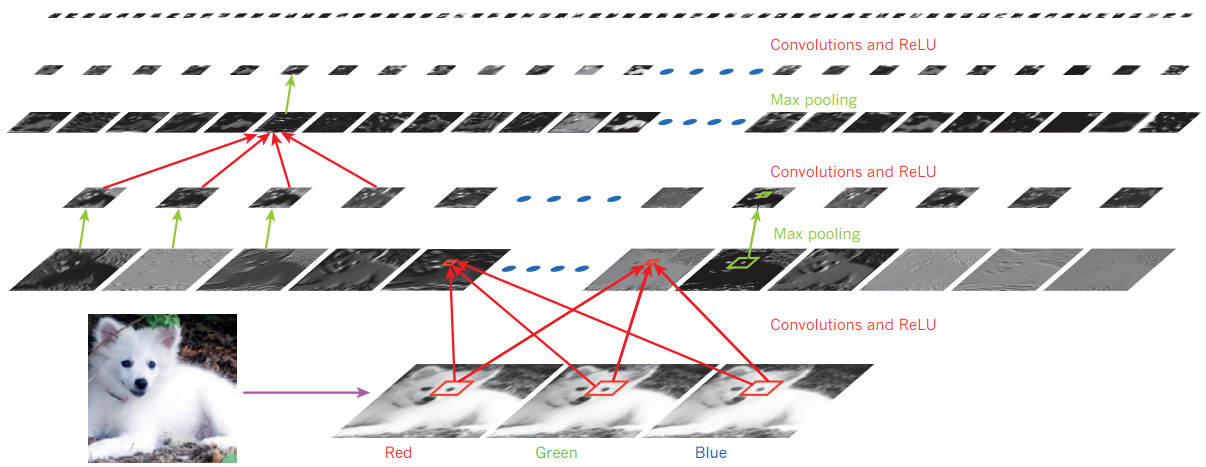
\includegraphics[width=1\textwidth]{BasicConvNet.png}
\caption{The outputs (not the filters) of each layer (horizontally) of a typical convolutional network architecture applied to the image of a Samoyed dog. Each rectangular image is a feature map corresponding to the output for one of the learned features (LeCun et al., 2015)}
\end{figure}

\noindent
The deep learning methods described so far are limited to returning one classification per image, however this is suboptimal for the analysis of camera trap images. In order to identify multiple objects, researchers train object detectors which segregate the image into regions that are passed through a CNN. Three approaches for object detection have recently grown in popularity. The first is Faster Region-CNN which intelligently segregates the image into approximately 2000 proposal regions and passes each through a CNN \cite{ren2017faster} (Figure 6). The second YOLO (You-Only-Look-Once) which divides an image into a grid of boxes, and passes each box through the network considering a series of predefined `anchors' relevant to the predicted shape and size classifications of interest \cite{redmon2016you}. Lastly is Single Shot Multibox Detector, which considers a set of default boxes and makes adjustments to these boxes during training to align over the objects of interest \cite{liu2016ssd}. Object detection methods have an additional objective function evaluation metric known as Intersection over Union (IOU), which returns performance as the area of overlap of the true and predicted regions divided by the entire area of the true and predicted regions \cite{nowozin2014optimal}. 
\newline

\begin{wrapfigure}{r}{0.5\textwidth}
  \begin{flushright}
    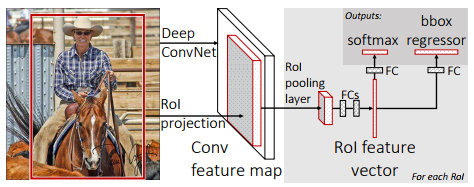
\includegraphics[width=3in]{FastRCNN.png}
  \end{flushright}
  \caption{Illustration of Fast R-CNN architecture (Girshick, 2015)}
\end{wrapfigure}

\noindent
In 2015, two research teams, Lisanti et al. and Martinel et al., demonstrated the successful capabilities of CNNs on human re-ID using the ETHZ data set, a data set composed of 8580 images of 148 unique individuals taken from mobile platforms, where CNNs were able to correctly classify individuals with 99.9\% accuracy after seeing 5 images of each individual and considering the most common model prediction as the final output \cite{lisanti2015person, martinel2015re}. Traditional CNNs for re-ID require large amounts of labeled data for each individual which is an infeasible requirement for animal re-ID. In 1993, Bromley et al. introduced a suitable neural network architecture for this problem, titled a Siamese network, which learns to detect if two input images that are similar or dissimilar \cite{bromley1994signature}. When considering re-ID, once trained, Siamese networks require only one labeled input image of an individual in order to accurately re-identify if an individual in a second image is the same. In 2015, Taigman et al. utilized a Siamese network for their system DeepFace which achieved a top-1 accuracy of 92.5\% on the YouTube Faces data set, a data set containing 3,425 videos of 1,595 individuals \cite{taigman2014deepface}. In 2016, Schroff et al. introduced FaceNet and a three image triplet loss objective function training similarity using input image as well as a similar and dissimilar image \cite{schroff2015facenet}. FaceNet currently holds the highest accuracy on the YouTube Faces data set with a 95.12\% top-1 accuracy \cite{schroff2015facenet}. 
\newline
\\
Based on the results for human re-ID, deep learning systems show promise as a generalizable framework for animal re-ID eliminating the biases related to human judgment and reducing the requirement for human labour to analyze images. With enough data, deep learning systems can be trained for any species which eliminates the need for domain expertise and species specific feature extraction algorithms. Deep learning systems also show promise to exceed human level performance when re-identifying animal individuals without obvious patterns and markings. 

\section*{Deep Learning for Camera Trap Analysis of Species and Animal Re-Identification}

Despite the success of deep learning methods for human re-ID, few ecological studies have utilized its advantages. In 2014, Carter et al.\ published one of the few works using neural networks for animal re-ID, a tool for green turtle (\textit{Chelonia mydas}) re-ID \cite{carter2014automated}. The authors highlight that green turtles have distinctive features on their shell and collected a variety of photos of 72 individuals, both nesting and free swimming, for their training and test set. Their pipeline initializes using a feature extraction method to pre-process the image by extracting a shell pattern, converting it to grey scale, unravelling the data into a raw input vector, and then training a simple feedforward network \cite{carter2014automated}. An average model produces an output accuracy of 80-85\% accuracy, but the authors train 50 different network and utilize an ensemble approach where each model votes and the final output is considered the most common classification. The ensemble approach returns an accuracy of 95\%. Carter et al.'s work has been considered a large success and is currently used on Lady Elliot Island in the southern Great Barrier Reef to monitor the green turtle population \cite{carter2014automated}. 
\newline
\\
In 2016, Freytag et al.\ trained the CNN architecture AlexNet on the isolated faces of chimpanzees considering the two publicly available data sets, C-Zoo and C-Tai \cite{freytag2016chimpanzee}. Freytag et al.\ (2016) report an improved accuracy of 92.0\% and 75.7\% in comparison to the original feature extraction method of 84.0\% and 68.8\% commenting how deep learning methods clearly outperform feature extraction methods for zoological applications involving identification \cite{freytag2016chimpanzee, loos2013automated}. In 2017, Brust et al.\ trained the object detection method YOLO to extract cropped images of Gorilla \textit{Gorilla gorilla} faces from 2,500 annotated images camera trap images taken in the Western Lowlands of the Nouabal\'e -Nodki National Park in the Republic of Congo \cite{brust2017towards}. Once the faces are extracted, Brust et al.\ (2017) followed the same procedure as Freytag et al.\ (2016) to train the CNN AlexNet to recognize individuals achieving a 90.8\% accuracy \cite{freytag2016chimpanzee, brust2017towards} (Figure 7). The authors close discussing how deep learning for ecological studies show promises for a whole realm of new applications if the fields of basic identify, spatio-temporal coverage and socio-ecological insights. \cite{freytag2016chimpanzee, brust2017towards}
\newline

\begin{figure}
  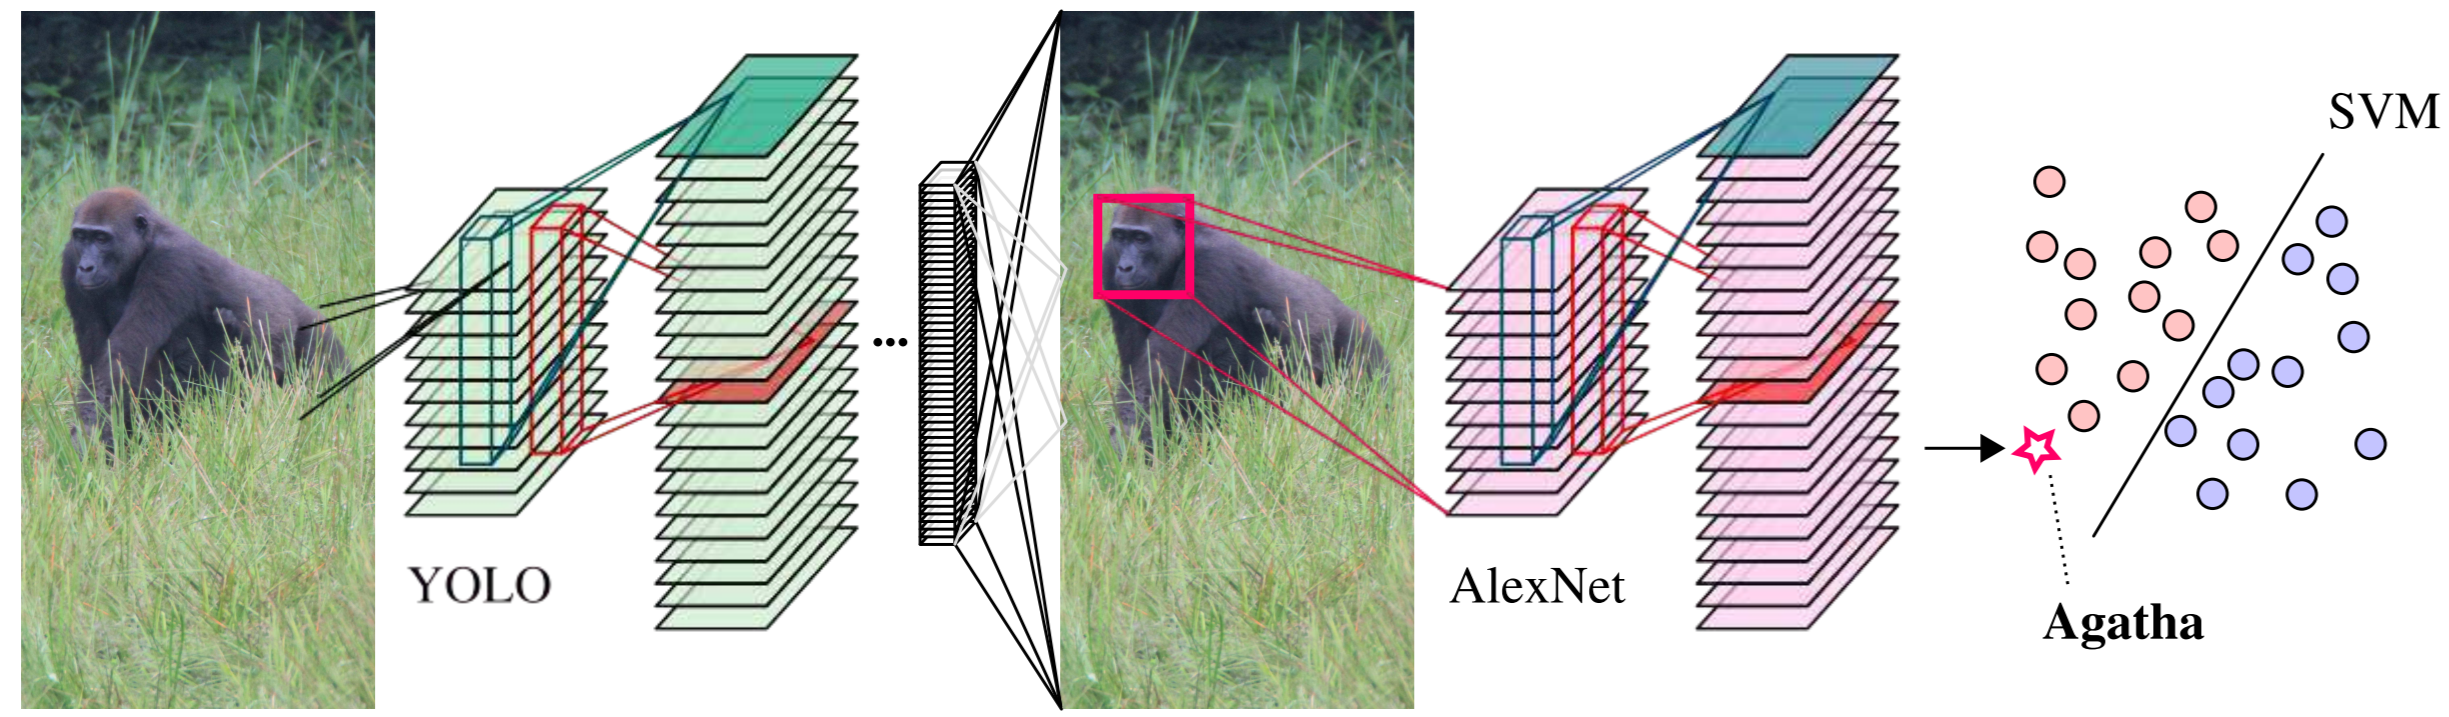
\includegraphics[width=6.5in]{GorillaRe-ID.png}
  \caption{Illustration of Pipeline used by Brust et al. using YOLO to extract facial images and an SVM to classify the individual (Brust et al., 2017)}
\end{figure}

\noindent
\newline
\\
Most recently, Deb et al. (2018) tested the re-ID capabilities of deep learning systems on three primate spieces: chimpanzees, lemurs (\textit{Lemuriformes spp.}), and golden monkeys (\textit{Cercopithecus kandti}) \cite{deb2018face}. Deb et al. (2018) consider three metrics for re-ID: verification (two image comparison), closed-set identification (individual is known to exist within the data), open-set identification (individual may or may not exist within the data) \cite{deb2018face}. For chimpanzees, Deb et al. (2018) combined the C-Zoo and C-Tai data sets to create the  \textit{ChimpFace} data set containing 5,599 images of 90 chimpanzees (Figure 8). For lemurs, they consider their own \textit{LemurFace} data set containing 3,000 face images of 129 lemur individuals from 12 different species. For golden monkeys, they extracted the faces of 241 short video clips (average 6 seconds) from Volcanoes National Park in Rwanda where 1,450 images of 49 golden monkey faces were cropped and extracted \cite{deb2018face}. Deb et al., (2018) use a custom CNN containing four convolutional layers, followed by a 512 node fully connected layer \cite{deb2018face}. The authors do not define the procedure for creating their similarity score metric, however my guess would be they use the Euclidean distance of the last feature layer considering each image. For the verification task they select two images and determine if the individuals are the same by considering if the similarity score is above a certain threshold. For the closed-set query they use this two image comparison approach first selecting an image and then cycling through the remaining database determining the same individual to be that with the largest similarity. Lastly, for open-set identification there is the added predisposition that the individual may not be within the data. To address this, they consider a similiarity threshold, where if all similarity scores are below this value there is no similar individual. Deb et al. (2018) train their network on large human face data sets and utilize transfer learning to initialize their model using these parameters. Deb et al. (2018) report considering verification, closed-set, and open-set respectively, for lemurs: 83.1\%, 93.8\%, 81.3\%, for golden monkeys: 78.7\%, 90.4\%, 66.1\% and for chimpanzess: 59.9\%, 75.8\%, and 37.1\% \cite{deb2018face}. 
\newline
\\
Before re-ID is possible, species ID must first occur reliably. Here I wanted to briefly highlight recent studies that have utilized deep learning to automate species identification from camera trap analysis. In 2016, Gomez et al. released two papers using deep CNNs for camera trap species recognition. The first compared 8 variations of the established the CNN frameworks AlexNet, VGG, GoogLeNet, and ResNet to train species classification on the Snapshot Serengeti data set, a dataset composed of 3.2 million camera trap images of 60 animal species, achieving a 88.9\% top one and 98.1\% top five accuracy \cite{gomez2016towards}. In 2016, Gomez et al. released a second paper aimed to utilize deep learning to improve low resolution animal species recognition by training deep CNNs on poor quality images \cite{gomez2016animal}. The data was labeled by experts into two data sets, the first classifying between bird and mammal and the second species classification of different mammal species. The authors claim to have reached an accuracy of 97.5\% and 90.35\% on the two classification tasks respectively \cite{gomez2016animal}. 
\newline
\\
In 2017, Norouzzadeh et al., used transfer learning to train six different deep convolutional network architectures (AlexNet, VGG, ResNet-50, ResNet-101, ResNet-152, and GoogLeNet) on a modified Snapshot Serengeti data set removing all images having multiple species (approximately 5\%), and images of species with low detection frequency \cite{norouzzadehautomatically}. Their best model achieved 92.1\% accuracy. The authors emphasize the time saving benefit of the technique and encourage further work into behaviour estimation, gender and age utilizing the data set's additional classifications. 
\newline
\\
In 2018, Schneider et al. addressed the limitation of traditional CNNs returning one classification output per image by comparing object detector models Faster R-CNN and YOLO for quantifying numerous species classifications from images where Faster R-CNN returned an accuracy of 93.0\% and 76.7\% on the Reconyx Camera Trap, a dataset of 936 images of 20 species, and the refined Gold Standard Snapshot Serengeti dataset respectively \cite{schneider2018deep}. The authors cite high class imbalance and densely populated images as the limiting factor for Snapshot Serengeti model.

\section*{Animal Re-Identification Species Data}

For my research, I propose implementing a pipeline of deep learning methods, specifically, object detection and similarity comparison, to build a successful application for animal re-ID. For my research I plan to test the deep learning methods on four species: Chimpanzee, Humpback Whale, Fruit Fly (\textit{Drosophila melanogaster}), and Octopus (\textit{Octopus vulgaris}). Each species and data set provide a unique challenge allowing for a robust analysis of the performance of my methodology. 
\newline
\\
To approach the problem of animal re-ID, the major limitation of traditional softmax classifiers is that the number of output classifications must be known. This is unrealistic when analyzing camera trap data. In order to solve this, I will train a Siamese network to learn animal similarity and that compares individuals from a known database. Upon initialization, this database is empty. As each individual enters into the camera, the network will query all existing animals within the database. If none are deemed to be similar, images of the new individual will be added to the database and the process repeats for each individual that enters. 
\newline
\\
To train the network required for this model I need to collect accurately labeled images of animal individuals and format the data appropriately for a Siamese network. Assuming for now I am given accurate images of animals from a publicly available data set, I repeat the following two steps for each individual to create an appropriate data set for training a similarity network. The first step is to assign all unique pairs of images of the same individual to an appropriate binary classification (Eg. 1 represent same). Then, for the number of the unique pairs created, I randomly select an image of the current individual as well as randomly select an image of an alternative individual and assign the appropriate binary classification (Eg. 0 represent different). To ensure training stability, I create an equal number of same and different classifications for each individual. 
\newline
\\
To measure the performance of a model, I consider the accuracy on a created validation and test set for each species. The validation data are created by randomly splitting the created pair data by a ratio of 1/10 split. This creates a data set of images seen during training, but in novel combinations. To test how well the model generalizes to individuals not seen during training, for each data set I create a test set by randomly excluding \~10\% of the individuals and create a similar pairwise data set for these unseen individuals. This second data set provides a better representation for how well the model generalizes to realistic scenarios of unseen individuals and is used as my primary metric. 
\newline
\\
For the re-ID of Chimpanzee, I will consider the publicly available C-Zoo and C-Tai data sets introduced by Loos and Ernst (2013) combined into the \textit{Chimpface} dataset introduced by Deb et al. (2018) \cite{loos2013automated, deb2018face}. This data set provides the unique opportunity of comparing the performance of similarity comparison models to the previously reported performance of feature engineering as well as deep learning methods. After following the described data creation format, the training set contains 148,516 pairs of images, the validation set 13,656 pairs of images, and the test set 16,398 pairs of images created by considering 8 random individuals not included in the training data.  
\newline

\begin{wrapfigure}{r}{0.5\textwidth}
  \begin{flushright}
    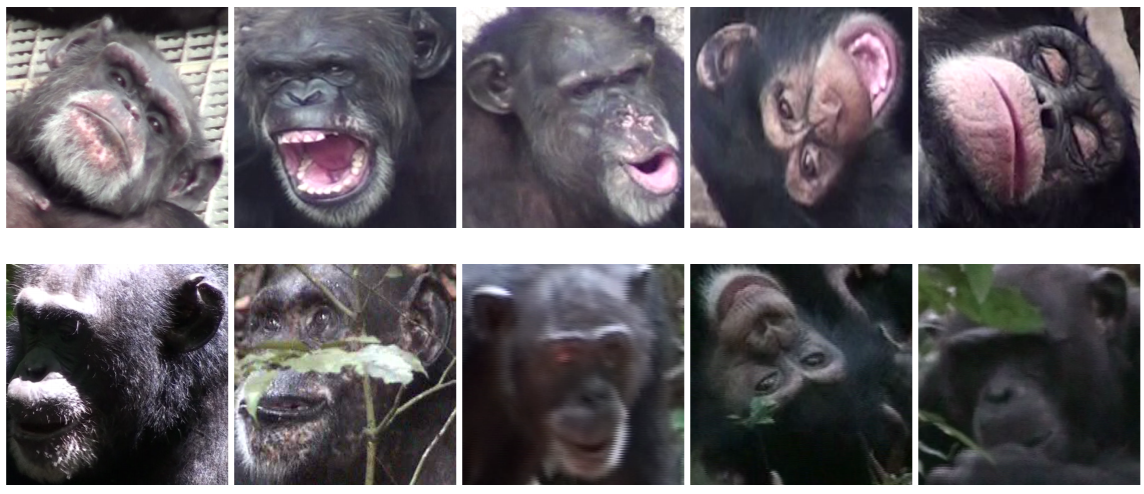
\includegraphics[width=3in]{ChimpanzeeExamples.png}
  \end{flushright}
  \caption{Example Images from C-Zoo and C-Tai Chimpanzee Data Sets}
\end{wrapfigure}

\noindent
To test re-identifying Humpback Whales, I will consider the Humpback Whale Identification Challenge data set offered as a Kaggle competition. This data set provides a realistic representation of the real world application of animal re-ID as the 9,046 images only contain the fluke of the whale and are extremely sparse, having only an average of only 2 (+/- 8) individuals considering 4,251 individual classifications (Figure 3). After creating the pairwise data, the training set has 25,399 image pairs, validation set 2,655 image pairs, and test set 3,822 image pairs. There are much fewer images because there are far less pair combinations for each individuals.
\newline
\\
To test the re-ID of Fruit Flies, I plan to consider an unpublished Fruit Fly data set in collaboration with John Schneider, a member of Dr. Graham Taylor's machine learning research group. John Schneider currently is sole possession of high resolution images of fruit flies however we hope to form a collaboration to test the resiliency of similarity networks on this species. A fruit fly re-ID system provides large research implications as it is a common research subject among laboratory research groups. 
\newline
\\
Lastly, to test the re-ID capabilities considering octopus I will be using video data provided by Stefan Linquist \cite{scheel2017second}. This data set provides the largest challenge as the final application requires an accurate object detector to identify octopus as they enter the video frame and a similarity comparison network to determine if this individuals has been previous seen before. The data required to train these models involves documenting the bounding box coordinates for each octopus in each frame of video to train the object detector as well as extract these isolated octopus images into labeled folders of unique individuals to train the similarity comparison network.
\newline
\\
To collect bounding box and extract images of octopus individuals, I have created a universally applicable video data extraction tool to streamline the process. The user begins by selecting their video of interest. The software then asks the user to place their mouse cursor at the top left corner of an object of interest (eg. octopus) and follow along while the video plays and it records the X\&Y position of the mouse cursor for every frame. The software then repeats the video for the user to follow the bottom right corner of the same object. The user can then select if there are additional objects and repeat/review the process until the video is fully labeled. The end result are the necessary files required for the two data formats: the bounding box coordinates per frame of each octopus individual used to train the object detector, and the extracted images of each octopus individual used to train the similarity network. A demo of this software is available at: https://youtu.be/YcTj0ayztA4.
\newline
\\
At this point in time I have labeled 16 short octopus videos with 3.5 average octopuses per video and an average length of 2:14 minutes. 3 videos are used to create the test set. I manually inspect each folder and delete approximately 90\% of images that appear redundant over time (ie. when an octopus remains stationary). I then follow the same Siamese data creation format as listed above for each video independently to create a current total of 80,916 training pairs, 9,080 validation pairs, and 17,968 unseen testing pairs. For each video the pairwise interactions are independently created as the identity across videos is uncertain.

\section*{Animal Re-Identification Methodology}

To approach the problem of animal re-ID, I propose the use of similarity networks as opposed to classification networks due to their previously described advantages. For my analysis I consider a network architecture composed of two sister networks based on the VGG16 architecture, consisting of 10 2-dimensional convolution layers and 4 max pooling layers \cite{simonyan2014very}. The features of the last convolution layer are then concatenated together, passed through two fully connected layers, and lastly through a binary output representing similar/dissimilar pairs. The model is shown paired examples of similar and dissimilar images and must modify its weights to output the correct binary classification (Figure 9). 
\newline

\begin{figure}
	\begin{center}
	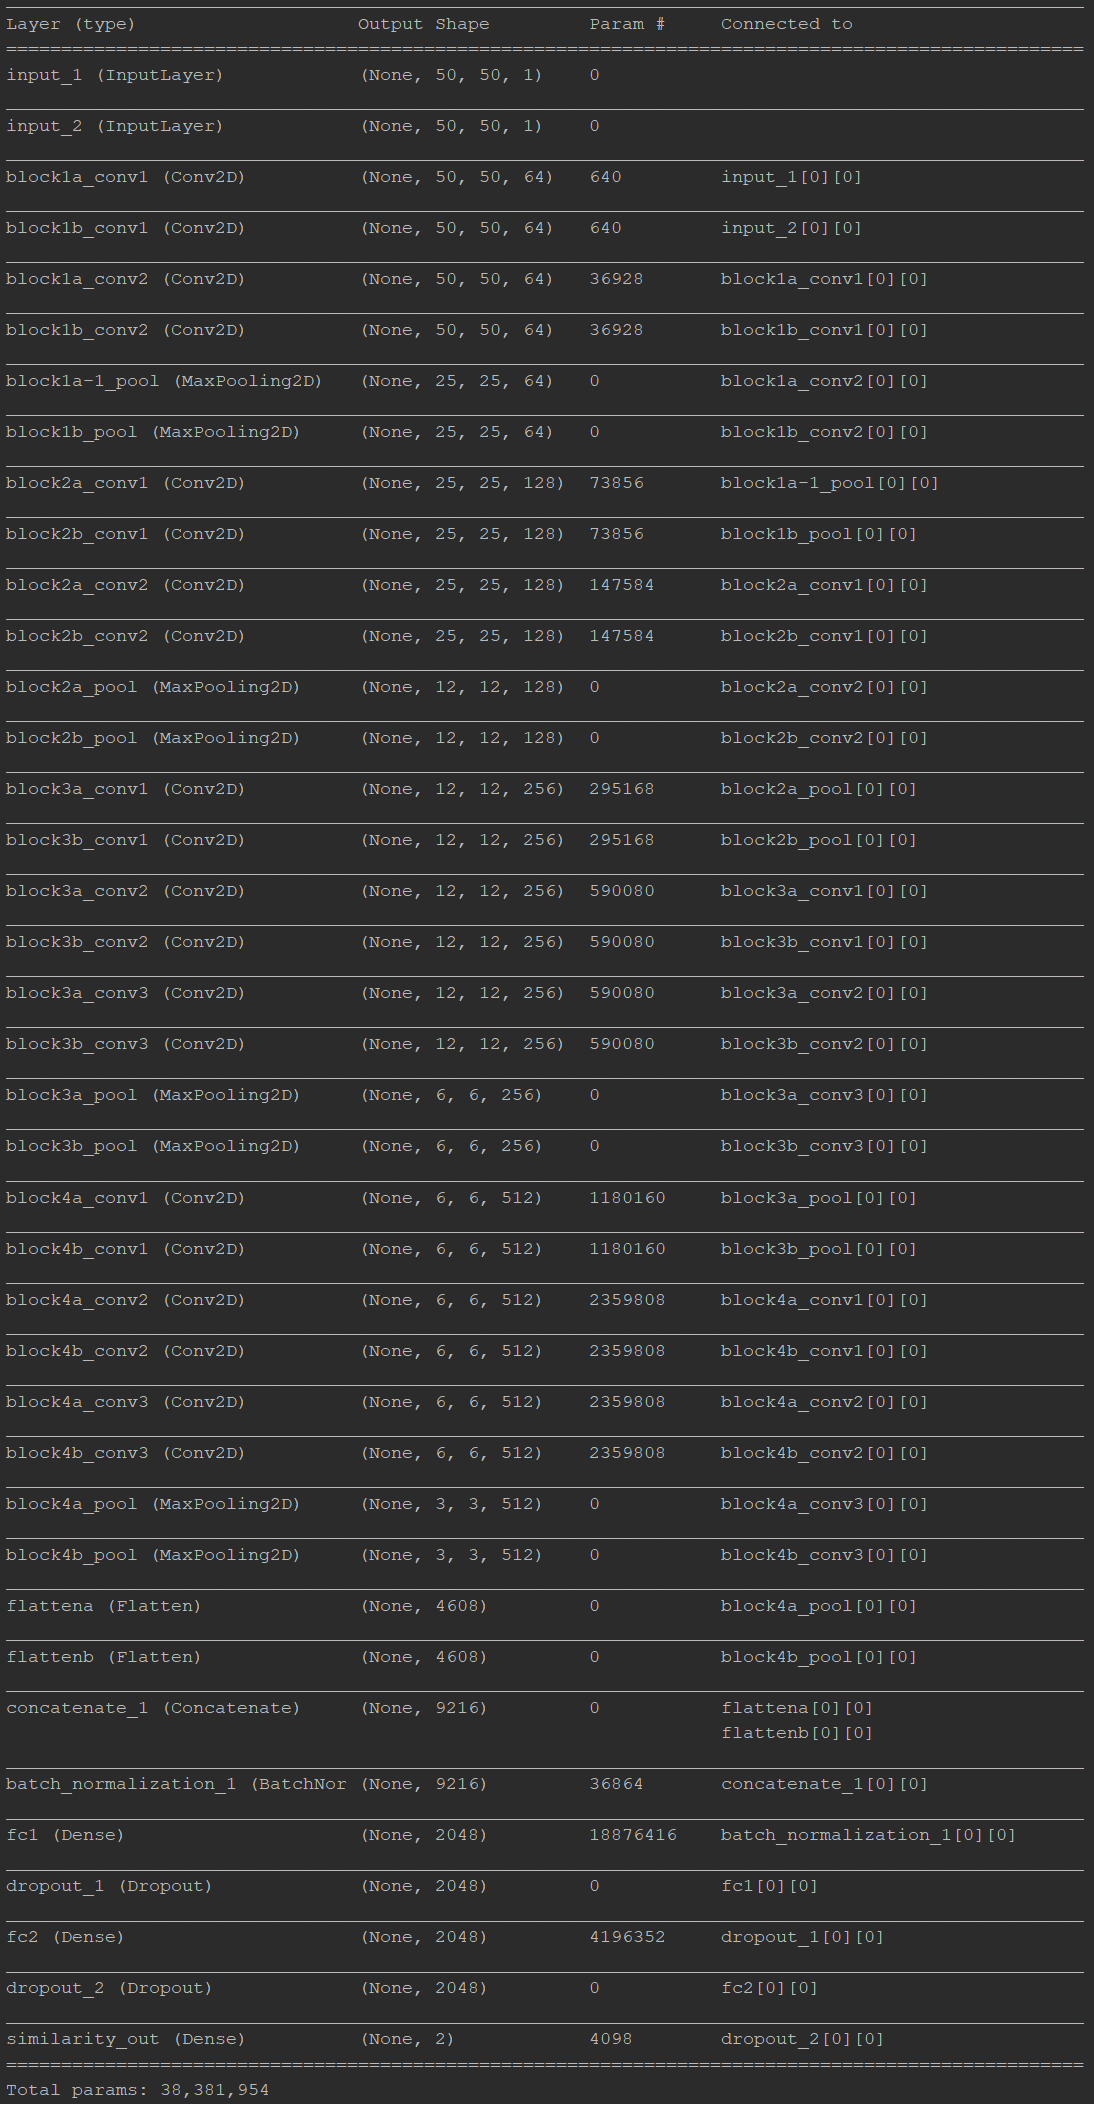
\includegraphics[width=4.8in]{ModelSummary.png}
	\caption{Detailed Siamese Network Model Description}
	\end{center}
\end{figure}

\noindent
In addition to the general architecture, I consider a variety of regularization techniques to improve training stability and prevent overfitting. I have found that initializing the model with the Xavier (also known as Glorot normal) initialization helps improve the likelihood of successful training as random initialization often stay in local minima \cite{glorot2010understanding}. Also, before each fully connected layers I implement batch normalization, a technique shown to help improve generalization of a model \cite{ioffe2015batch}. To prevent overfitting, I also regularize the final two fully connected layers with a Ridge regression value of 0.01 which penalizes the complexity of the function by including a squared error term that the model must also minimize \cite{hoerl1970ridge}. I also include a 50\% dropout for both fully connected layers which for each mini-batch randomly prohibits the use of 50\% of the nodes in the fully connected layers \cite{srivastava2014dropout}.
\newline
\\
In addition to these techniques, to help improve generalization I also apply data augmentation methods during training. For every training example, there is a given probability that the image will be modified in some capacity while maintaining the correct labels. This technique helps improve generalization and reduce overfitting as it artificially creates additional training examples. For each training example I set a 50\% chance that the image is flipped along the horizontal axis, a random direction horizontal shift up to 20\% the image size, a random direction vertical shift up to 20\% the image size, a random zoom location and value considering 20\% the image size, and lastly a random rotation direction and orientation up to 20 degrees from the vertical axis. When performing data augmentation, when the image is shifted or rotated beyond the scope of the original image, black pixels are added to the empty locations. 
\newline
\\
To train the weights of the neural network I select the Adaptive Momentum (Adam) optimizer with a learning rate of 0.001 \cite{kingma2014adam}. Simply stated, Adam is regarded as the most universally applicable optimizer, capable of increasing and decreasing its step size relevant to the speed at which the error is decreasing and also adjusting its direction travel to the steepest descent similar to RMS Prop \cite{kingma2014adam}. To represent error, I consider the binary crossentropy loss considering the binary output of the similarity network. I train the model using mini-batch sizes of 128 training examples. As a metric for recording performance during training, I consider the accuracy on the test set of previously unseen individuals and only save the model if the current epoch is an improvement over the previous. In essence, this approach allows me to consider early stopping as a means of regularization and selects the model which best generalizes to unseen individuals. Lastly, I train the model for 100 epochs. Training and analyses of this model were performed using Python 3.6, Tensorflow 1.8, and Keras 2.2 using two GPUS: NVidia 1080 GTX and NVidia 680 GTX. 

\section*{Results}

At this point in my research, I have performed analyses on the \textit{Chimpface}, Kaggle whale data set, as well as preliminary octopus results.
\newline
\\
Considering the \textit{Chimpface} data set, the training set outputs an accuracy of 88.2\% and the validation set containing 16,398 pairs of images of individuals previously seen during training, outputs an accuracy of 87.5\%. The test set containing 13,656 pairs images where the model is predicting the similarity of individuals never seen by the model, the model outputs an accuracy of 75.5\% (Figure 10, 11 \& 12). This is a large improvement over the verification score of 59.9\% using the same data reported by Deb et al. (2018) \cite{deb2018face}.
\newline
\\
Considering the humpback whale data set, the model returns a highest performing test accuracy of 61.4\% and validation accuracy of 62.3\%. In fact, when overfitting, the train accuracy of the model only achieves 65.2\%. This suggests that the model is not complex enough to capture the representation of whale individuals, which is unlikely considering its success on \textit{Chimpface}. An alternative explanation is that the despite the data augmentation techniques, this data set is too limited for my current deep learning architecture having on average only 2 or 3 pairs of similar images (Figure 13).
\newline
\\
Fruit fly data and results coming soon.
\newline
\\
Considering the created octopus data set, the model returns a training accuracy of 97.8\%, validation accuracy of 95.3\% and testing accuracy of 92.2\% considering octopus it hasn't seen during training (Figure 14 \& 15). These results show promise considering more data can still be collected. Pushing to achieve greater than 95\% accuracy seems like a tangible objective. 
\newline
\\
Lastly, to create the final animal re-ID application, I have trained a Faster R-CNN model using the Inception architecture with a 96.4\% accuracy when predicting regions containing octopus with an IOU value of 0.82. A video demo is available at: https://www.youtube.com/watch?v=TXbv5pN4JRI. Current analysis takes approximately 8 hours for 3 minutes of footage which is too slow for any practical use on long term video analysis. My next step is to train a YOLO object detector to take advantage of its near 63x increased speed over Faster R-CNN \cite{redmon2016you}. Once a YOLO model is trained, the final steps include piecing together the object detector and similarity comparison network to complete the re-ID application. Once completed I plan to use it for long term octopus video analysis and perform an ethological analysis on octopus behaviour.
\newline
\\

\section*{Near Future Techniques for Animal Re-Identification}
Ecologists familiar with techniques in computer vision have exhibited considerable ingenuity in developing feature extraction methods for animal re-ID, but few have considered modern deep learning methods, such as CNNs or Siamese networks. Advantages that are commonly associated with feature detection approaches include increased accuracy, reduced biases related to human judgments, and reduced labour costs. However these advantages are limited to organisms with conspicuous individual differences, as well as researchers who possess sufficient expertise to identify those features and program systems capable of detecting them. By considering modern deep learning approaches, ecologists can utilize these advantages without the requirement of hand-coded feature extraction methods by training a neural network to learn these features, or others we had no prior knowledge about, from large amounts of data. 
\newline
\\
While limited within the field of ecology, deep learning approaches have shown great success re-identifying human individuals considering only a single image for reference when using a network designed for similarity comparisons when trained on large amounts of data. We foresee the creation of labeled datasets for numerous animal individuals as the largest hurdle for deep learning approaches for animal re-ID. Our proposed approach for data collection would be to utilize environments with known ground truths for individuals, such as zoos or camera traps in combination with individuals being tracked by GPS, to build the datasets. We would recommend using video wherever possible to gather the greatest number of images for a given encounter with an individual. To reduce the labour for manual cropped image extraction, we would recommend training an object detector and combining it with simple tracking to autonomously extract cropped and labeled images of individuals from video. We encourage researchers with images of labeled animal individuals to make these datasets publicly available to further the research in this field.
\newline
\\
When considering the deployment of a machine learning systems, the earliest approach may be to manually collect the data storage devices from the cameras after a given period of time and pass the images through a network for analysis when returning to a central or cloud computer. As confidence in these systems builds, there is an opportunity to embed the analysis within the cameras themselves similar to other mobile devices. This approach provides numerous advantages. The first includes sending the results from the camera trap analysis wirelessly, if reception available, so researchers do not have to regularly visit the site. The latter provides a benefit to storage, especially considering video, as the camera would be able to analyze the environment without the need to store information on the device also decreasing the frequency of visits. 
\newline
\\
While deep learning approaches are able to generalize to examples similar to those seen during training, we foresee various environmental, positional, and timing related challenges. Environmental difficulties may include challenging weather conditions, such as heavy rain, or extreme lighting/shadows. A possible solution to limit these concerns may be to re-ID only during optimal weather conditions. A positional challenge may occur if an individual were to enter the camera frame at extremely near or far distances. To solve this, one could limit animals to a certain range from the camera before considering it for re-ID. Lastly, a challenge may be if an individual's appearance were to change dramatically between sightings, such as being injured or the rapid growth of a youth. While a network would be robust to such changes given training examples, this would require examples be available as training data. 
\newline
\\
The development of a computer vision method for animal re-ID have aided in the autonomous and unbiased population estimation. If deep learning systems can demonstrate accurate animal re-ID at a similar success to humans, one could utilize these methodologies to create systems that autonomously extract a variety of ecological metrics such as diversity, evenness, richness, relative abundance distribution, carrying capacity, and trophic function, contributing to larger overarching ecological interpretations of trophic interactions and population dynamics.
\newline
\\
\section*{Conclusion}
Population estimates are the underlying metric for many fundamental ecological questions and rely on the accurate re-identification of animals. Camera and video data have become increasingly common due to their relatively inexpensive method of data collection, however they are criticized for their unreliability and bias towards animals with obvious markings. Feature engineering methods for computer vision have shown success re-identifying animal individuals and removing biases from these analyses, however these methods require algorithms designed for feature extraction. Deep learning provides a promising alternative for ecologists as it learns these features from large amounts and has shown success for human re-ID. By utilizing deep learning methods for object detection and similarity comparison, ecologists can utilize deep learning methods to autonomously re-identify animal individuals from camera trap data. Such a tool would allow ecologists to automate population estimates.

\newpage
\begin{table}[h!]
\centering
\caption{A summary of the feature engineering and feedforward network learning methods for animal re-identification. All of these studies use different test sets and so this table should not be considered as a comparison of the performance of the methodologies.}
\begin{tabular}{ l c l c c }
	\multicolumn{5}{ c }{Computer Vision Animal Re-Identification Techniques}\\
	\hline
	Animal & Year & \centering{Methodology} & Test Size & \multicolumn{1}{p{2.5cm}}{\centering Top-1 \\ Accuracy (\%)} \\ \hline
	Sperm Whale & 1990 & Database similarity & 56 & 59 \\
	Humpback Whale & 1990 & Database similarity & 30 & 41.4 \\
	Grey Seal & 1990 & 3-D Pattern Cell similarity & 56 & 98.0 \\
	Sperm Whale & 1998 & Wavelet transformations & 56 & 92.0 \\
	Cheetah & 2001 & 3-D Pattern Cell similarity & 10,000 & 97.5 \\
	Whale/Dolphin & 2003 & XY Pair Euclidean Distance & 23-127 & 50.0 \\
	Marbled Salamander & 2004 & Pixel histogram and local colours & 69 & 72.0 \\
	Whale Shark & 2005 & Star pattern recognition & 236 & 90.0 \\
	Elephant & 2007 & Polynomial multi-curve matching & 200 & 75.0 \\
	Tiger & 2009 & 3-D Pattern Cell similarity & 298 & 95.0 \\
	African penguin & 2010 & Per feature AdaBoost classifer & N/A & 92-97.0 \\
	Zebra & 2011 & Pixel histogram similarity & 85 & 50.0 \\
	Manta Ray & 2013 & Colour histograms & 720 & 51.0 \\
	Chimpanzee (C-Zoo) & 2013 & Support Vector Machine & 422 & 84.0 \\
	Chimpanzee (C-Tai) & 2013 & Support Vector Machine & 1016 & 68.8 \\
	Green Turtule & 2014 & Feedforward Network & 72 & 95.0 \\
	Chimpanzee (C-Zoo) & 2016 & Convolutional Network & 422 & 92.0 \\
	Chimpanzee (C-Tai) & 2016 & Convolutional Network & 1016 & 75.7 \\
	Shark & 2017 & Naive Bayes Nearest Neighbour & 2371 & 82.0 \\
	Gorilla & 2017 & Convolutional Network & 2000 & 90.8 \\

\end{tabular}
\end{table}


%\newpage
%\begin{table}[h!]
%\centering
%\caption{A summary of the feature engineering and feedforward network learning methods for animal re-identification. All of these studies use different test sets and so this table should not be considered as a comparison of the performance of the methodologies.}
%\begin{tabular}{ l c c c }
%	\multicolumn{4}{ c }{Computer Vision Animal Re-Identification Techniques}\\
%	\hline
%	Data & Train Accuracy & Val Accuracy & Test Accuracy \\
%	C-Tai & 99 & 98 & 70 \\
%	C-Zoo & 99 & 98 & 70 \\
%	C-Tai and C-Zoo & 99 & 98 & 70 \\
%\end{tabular}
%\end{table}

\newpage


\begin{figure}
    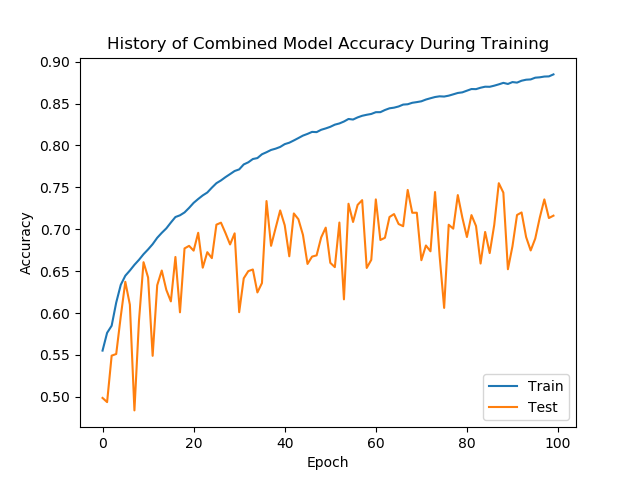
\includegraphics[width=17cm]{ChimpAcc.png}
  \caption{Chimpanzee Accuracy}
\end{figure}

\begin{figure}
    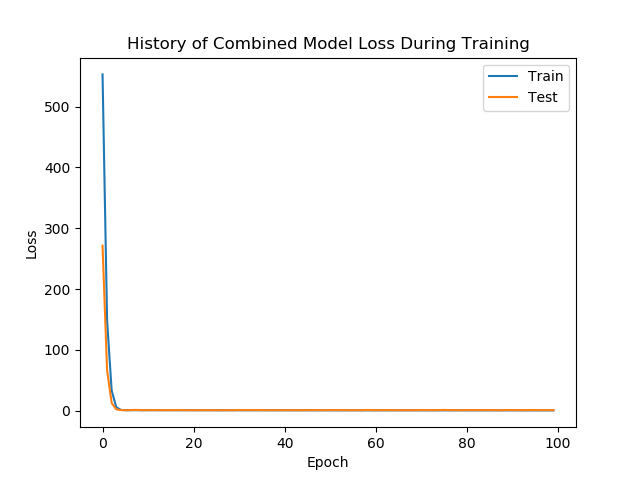
\includegraphics[width=17cm]{ChimpLoss.png}
  \caption{Chimpanzee Loss}
\end{figure}

\begin{figure}
	\begin{center}
    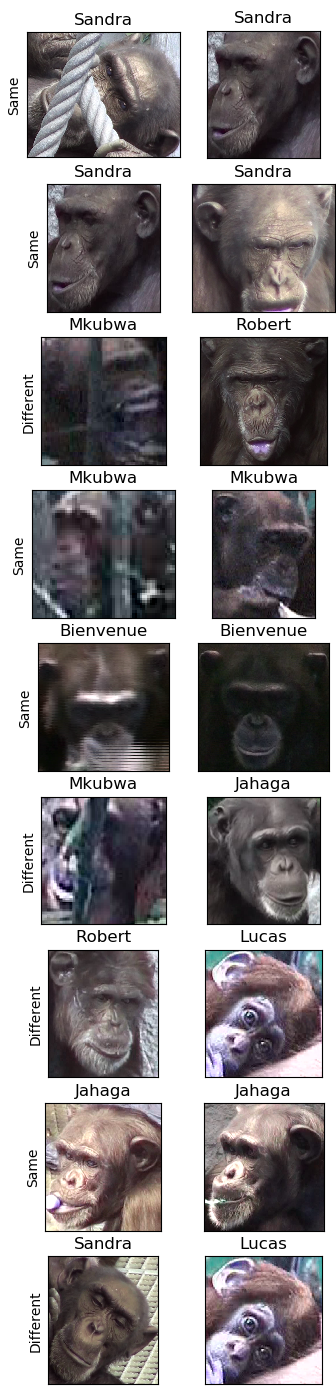
\includegraphics[width=2.0in]{ChimpanzeeComparison.png}
  \caption{Model Output for Chimpanzee Individuals}
  	\end{center}
\end{figure}

\begin{figure}
    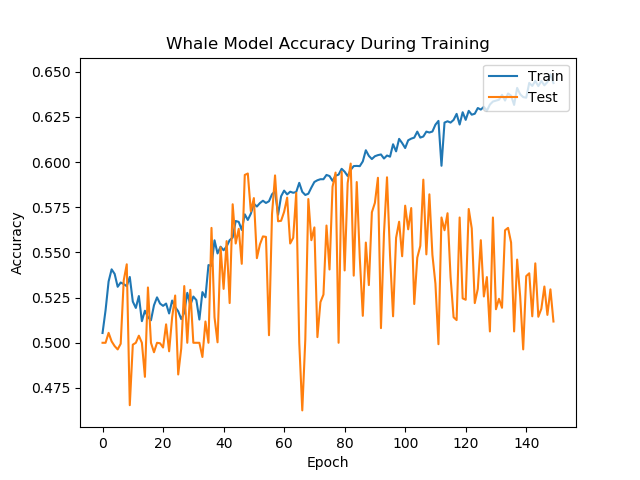
\includegraphics[width=17cm]{HumpbackWhaleAccuracy.png}
  \caption{Humpback Whale Accuracy}
\end{figure}

\begin{figure}
    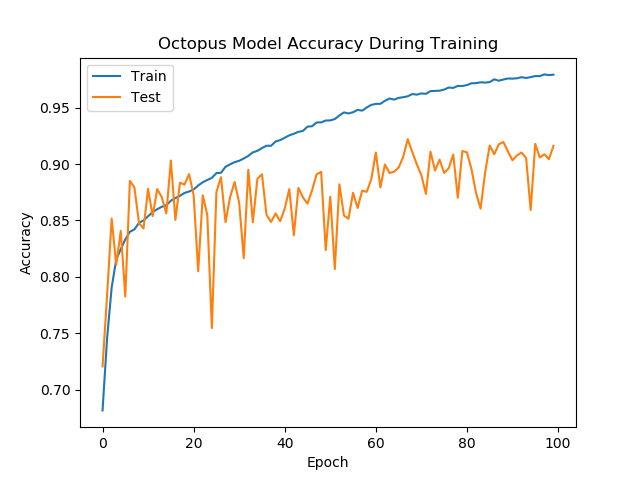
\includegraphics[width=17cm]{OctopusAccuracy.png}
  \caption{Octopus Accuracy}
\end{figure}

\begin{figure}
    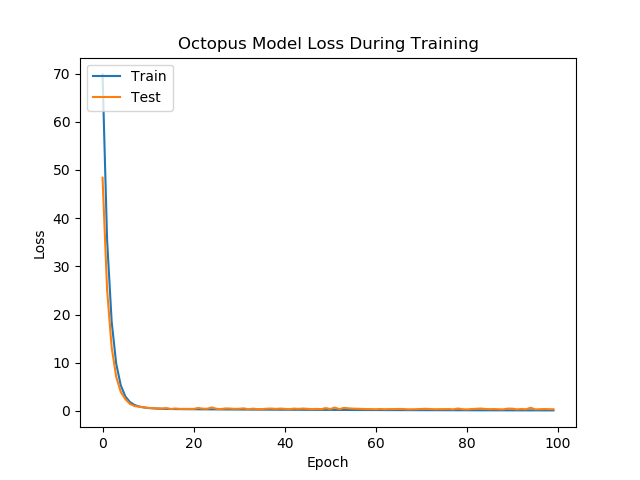
\includegraphics[width=17cm]{OctopusLoss.png}
  \caption{Octopus Loss}
\end{figure}

\begin{figure}[t!]
	\centering
	\textbf{Time Line of Computer Assisted Approaches}\par
	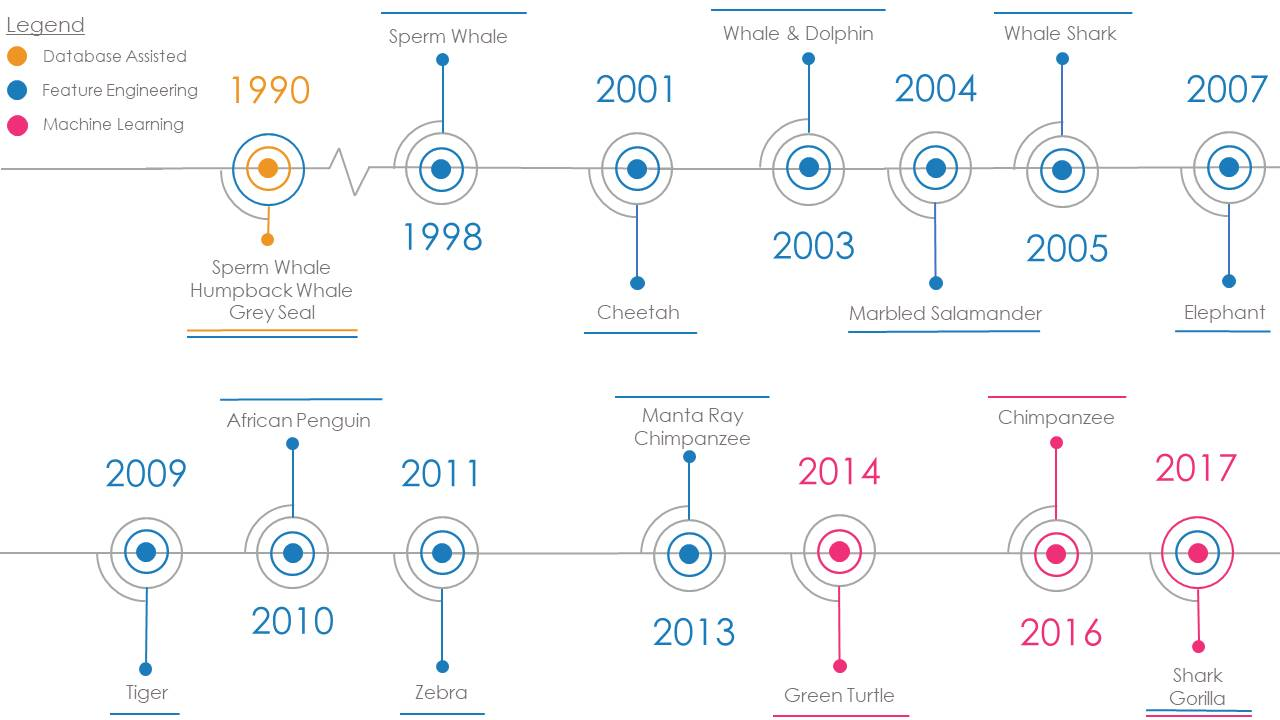
\includegraphics[width=17cm]{SpeciesTimeLine.jpg}
	\caption{A time line of the computer assisted animal species re-identification methods discussed in this review segregated into Database Assisted, Feature Engineering, and Machine Learning}
\end{figure}


\clearpage
\bibliographystyle{IEEEtran}
\bibliography{MasterReference}



\end{document}

